\documentclass[10pt]{article}
\usepackage[polish]{babel}
\usepackage[utf8]{inputenc}
\usepackage[T1]{fontenc}
\usepackage{amsmath}
\usepackage{amsfonts}
\usepackage{amssymb}
\usepackage[version=4]{mhchem}
\usepackage{stmaryrd}
\usepackage{graphicx}
\usepackage[export]{adjustbox}
\graphicspath{ {./images/} }

\title{LIGA MATEMATYCZNA \\
 im. Zdzisława Matuskiego \\
 STYCZEŃ 2023 \\
 SZKOEA PONADPODSTAWOWA }

\author{}
\date{}


\begin{document}
\maketitle
\section*{ZADANIE 1.}
Liczby \(1,2,3, \ldots, 9\) umieszczono na okręgu. Przez operację rozumiemy dodanie pewnej (tej samej) liczby całkowitej do dwóch wybranych sąsiednich liczb i umieszczenie tych sum na okręgu w miejsce poprzednich liczb. Czy po wykonaniu skończonej liczby takich operacji można otrzymać na okręgu dziewięć zer?

\section*{ZADANIE 2.}
Czy używając wszystkich dziesięciu cyfr można ułożyć liczbę podzielną przez 11?

\section*{ZADANIE 3.}
Na boku \(A B\) kwadratu \(A B C D\) wybrano punkt \(E\), a na boku \(B C\) wybrano punkt \(F\) i połączono je z wierzchołkami kwadratu. Odcinki te podzieliły kwadrat na osiem części. Na rysunku zapisano pola trzech z nich. Oblicz pole zaznaczonego czworokąta.\\
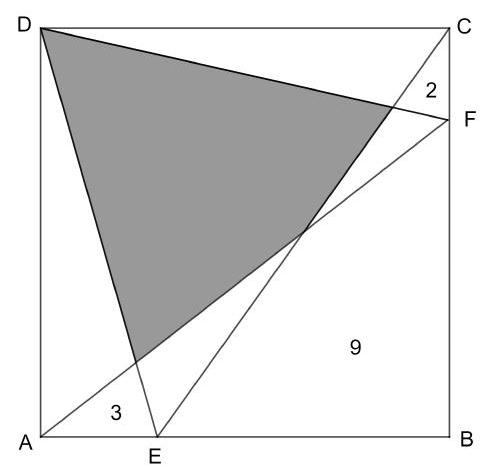
\includegraphics[max width=\textwidth, center]{2024_11_21_f70f11ddd7e367b8e73ag-1}

\section*{ZADANIE 4.}
W zbiorze liczb rzeczywistych rozwiąż układ równań

\[
\left\{\begin{array}{l}
2 x+3 y=5 y^{2} \\
2 y+3 x=5 x^{2}
\end{array}\right.
\]

\section*{ZADANIE 5.}
Wyznacz wszystkie liczby pierwsze \(p\) o tej własności, że \(p+11\) jest dzielnikiem liczby

\[
p(p+1)(p+2)
\]


\end{document}